\part{Matrices}
\frame{\partpage}

\begin{frame}
	\begin{center}
		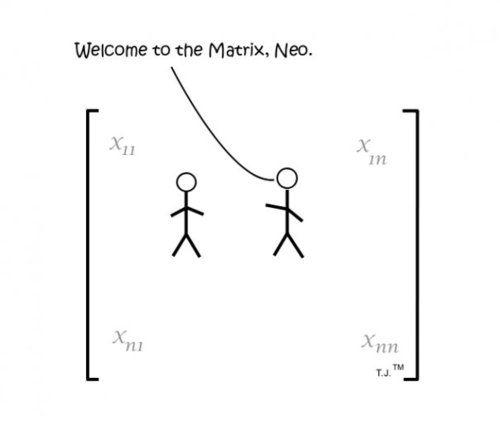
\includegraphics[height=0.8\textheight]{matrixjoke}
	\end{center}
\end{frame}

\begin{frame}{Matrices}
	\begin{itemize}
		\pause\item An $m \times n$ \textbf{matrix} is a rectangular array of numbers, having $m$ rows and $n$ columns
		\pause $$
			\begin{pmatrix}
				3 & 0 & 2.4 \\
				1.7 & -6 & -4.5
			\end{pmatrix}
			\qquad \leftarrow \text{A $2 \times 3$ matrix}
		$$
		\pause\item Note: the plural of \textbf{matrix} is \textbf{matrices}
		\pause\item In computer graphics we mostly work with \textbf{square} matrices (number of rows = number of columns)
	\end{itemize}
\end{frame}

\begin{frame}{Multiplying vectors and matrices}
	\begin{itemize}
		\pause\item Two $n \times n$ matrices can be \textbf{multiplied}, giving a new $n \times n$ matrix
		\pause\item An $n \times n$ matrix and an $n$-vector can be \textbf{multiplied}, giving a new $n$-vector
		\pause\item See \url{https://www.khanacademy.org/math/precalculus/precalc-matrices/multiplying-matrices-by-matrices/v/matrix-multiplication-intro}
		\pause\item (But you don't really need to know how to calculate these manually...)
	\end{itemize}
\end{frame}

\begin{frame}{Commutativity}
	\begin{itemize}
		\pause\item Multiplication of numbers is \textbf{commutative}
			\begin{itemize}
				\pause\item $a \times b = b \times a$
				\pause\item e.g.\ $2 \times 3 = 3 \times 2$
			\end{itemize}
		\pause\item Multiplication of matrices is \textbf{not commutative}
			\begin{itemize}
				\pause\item In general, $A \times B \neq B \times A$
				\pause\item There may be some matrices where $A \times B = B \times A$, but they are the exception
			\end{itemize}
	\end{itemize}
\end{frame}

